\documentclass[journal]{IEEEtran}
\usepackage{amsmath,amssymb,amsthm,bm}
\usepackage{booktabs,multirow}
\usepackage{graphicx}
\usepackage{xcolor}
\usepackage{url}
\usepackage[hidelinks]{hyperref}
\usepackage{microtype}
\usepackage{placeins}
\usepackage[fontset=fandol]{ctex}
\graphicspath{{../figures/final/}}
\makeatletter
\setlength{\@fptop}{0pt}
\setlength{\@fpsep}{12pt}
\setlength{\@fpbot}{0pt plus 1fil}
\setlength{\@dblfptop}{0pt}
\setlength{\@dblfpsep}{12pt}
\setlength{\@dblfpbot}{0pt plus 1fil}
\makeatother
\renewcommand{\topfraction}{0.95}
\renewcommand{\floatpagefraction}{0.80}
\title{scVICAR：用于掩码单细胞表征学习的有界图邻域锚点恢复}
\author{匿名作者\thanks{用于双盲评审的中文阅读稿。投稿与引用以英文正式稿为准。}}
\begin{document}
\maketitle

\begin{abstract}
掩码自编码器通过重建被替换的基因值来学习单细胞表征。scMAE 的替换过程主要利用细胞内部的基因信息，细胞之间的局部关系尚未参与训练。我们提出 scVICAR：先将一个细胞与其近邻轻微混合，再要求模型恢复原始细胞。scVICAR-F 对所有细胞使用固定混合系数；scVICAR-T 根据局部图结构调整邻边权重和逐细胞混合系数。统一算子保持局部凸包，并给出输入与表征扰动上界。它也可以写成一步非均匀图扩散。污染上界描述了跨类别邻居对扰动大小的影响。

在包含 15 个数据集、17 个完整方法配置和 765 次运行的开发阶段基准中，scVICAR-T 和 scVICAR-F 在 ACC、NMI、ARI 和 macro-F1 四项平均指标上分别位列第一和第二；相对 scMAE 的平均 ARI 提升分别为 5.08\% 和 3.93\%。在另行冻结的六数据集协议下，scVICAR-T 的平均 ARI 为 0.617，是所有比较方法中的最高值，比 Original scMAE 高 2.13\%。骨干完全一致时，平均效应更小并随数据集变化。受控错误邻边替换显示，拓扑信息亲和度识别跨类别边的平均 AUROC 为 0.918；逐细胞混合系数与邻域纯度的平均 Spearman 相关系数为 0.520。低标签量探针在多数数据集上略有改善，相对增益为 0.13\%–0.34\%；标记基因相关指标随数据集变化较大。

scVICAR 在本研究的开发数据和冻结数据上具有竞争力。拓扑自适应组件能够识别不可靠邻边，其聚类收益取决于数据集和图结构。
\end{abstract}
\begin{IEEEkeywords}
单细胞 RNA 测序；掩码自编码器；图表征学习；邻域风险；聚类；细胞类型注释。
\end{IEEEkeywords}
\section{1. 引言}

单细胞 RNA 测序（scRNA-seq）能够在细胞分辨率上测量转录组。后续分析需要表征同时保留生物学身份并抑制技术变异。表达矩阵具有稀疏、高维、测序深度差异大和类别不平衡等特点。表征空间中的错误可能合并稀有群体，或将连续的生物学程序错误分割。因此，可靠的表征学习同时决定细胞聚类和后续注释的质量。

深度生成模型和自编码模型能够直接从表达谱中学习非线性结构。掩码自编码提供了一种直接的自监督目标：模型替换观测的一部分，然后恢复原始内容。scMAE 将这一原则应用于 scRNA-seq，通过基因值替换、掩码预测和表达重建来学习表征。该过程主要利用细胞内部的基因上下文，细胞间关系尚未参与训练。

细胞间关系可以提供结构化训练信号。由表达数据估计的最近邻图也可能跨越细胞类型、技术批次、过渡状态和稀有群体边界。因此，局部混合需要同时控制每个细胞的移动幅度，并记录不可靠邻居对结果的影响。

为此，我们提出 single-cell Vicinal Corruption with Anchor Recovery（scVICAR）。它利用局部细胞几何构造训练输入，并始终恢复原始细胞。设 $\widehat P$ 为行随机的采样邻域算子，$G$ 为逐细胞混合系数构成的对角矩阵，则

\begin{equation}
X^v=(I-G)X+G\widehat PX=X-G(I-\widehat P)X.
\end{equation}

所得邻域视图随后接受原始的基因替换破坏。干净 scMAE 分支始终保留，最终 embedding 由干净表达谱直接提取，不需要在推理阶段进行图传播。这与同时插值输入和预测目标的 mixup 不同。

scVICAR-F 对所有细胞使用相同混合系数。scVICAR-T 根据余弦相似度、互惠 KNN 和共享邻居重叠计算邻边权重，并根据局部图一致性设置逐细胞混合系数。该亲和度是未经校准的解析权重。局部图一致性较弱时，scVICAR-T 减少混合量。

每个邻域视图均位于锚点细胞及其采样邻居构成的凸包内，其位移由局部半径和逐细胞混合系数共同限制。同一算子也可以看作一步非均匀图扩散。污染上界给出了跨类别邻居质量与扰动大小之间的关系，压力实验直接测量这些量。

实验采用三层证据结构。第一层是广泛的开发阶段基准，用于检验方法在不同数据上的总体竞争力。第二层是在六个此前未使用的数据集上进行冻结评估，并同时比较外部基线和骨干匹配对照。第三层通过错误邻边干预、组件消融、标记基因任务和低标签量探针检验机制及生物学效用。统计分析以数据集为独立单位，不选择最佳随机种子。真实标签不进入干净训练、图构建和参数选择，只用于最终评价及明确隔离的压力实验。

本文贡献如下：

\begin{enumerate}
\item 提出图邻域锚点恢复，以局部细胞几何构造有界输入破坏，并始终保持原始细胞为自监督目标。
\item 将拓扑自适应拆分为边亲和度与逐细胞混合系数，并分别进行组件消融和图污染实验。
\item 推导凸包、扰动、扩散和污染性质，并在受控图污染实验中检验相应量。
\item 建立分层评价体系：开发基准在 15 个数据集上比较 17 个完整方法配置，外部验证使用 6 个另行冻结的数据集，并进一步进行骨干匹配消融、图压力测试和防标签泄漏的下游任务。
\end{enumerate}

\section{2. 相关工作}

\subsection{2.1 单细胞表征与聚类}

标准单细胞流程通常先对表达矩阵降维，再构建细胞图并使用 Leiden 等社区发现算法。这类方法具有良好的可扩展性和可解释性，但结果会受到预处理、邻居数量、分辨率和初始几何的影响。深度方法则直接学习这一几何结构。scVI 使用概率潜变量模型；scDeepCluster 和 scDCC 将非线性表征与聚类结构结合；scGNN、scDSC 等图方法通过神经网络目标传播结构信息；scNAME 和 AttentionAE-sc 则引入邻域对比、掩码估计或注意力机制。这些工作说明细胞间上下文具有价值，同时也使模型更加依赖估计图或伪标签结构。

掩码自编码不需要在表征学习阶段指定聚类目标。scMAE 替换基因值、预测实际发生的掩码，并重建原始表达向量。scVICAR 保留这一骨干及其干净细胞目标，仅使用细胞图定义额外的破坏分布，再从该分布产生的视图中恢复原始锚点。

\subsection{2.2 邻域学习与图风险}

邻近细胞常共享细胞类型、状态、谱系或功能，因此细胞图非常有用。然而，稀疏性、类别不平衡、批次效应和图构建所依赖的投影都可能产生错误或不对称的边。反复传播还可能收缩有信息量的图频率成分，造成边界模糊和过平滑。稀有细胞尤其容易受到影响，因为其同类邻居更少。

scVICAR 使用细胞图构造训练输入，推理时直接编码干净表达谱。边亲和度决定不同邻居的贡献，逐细胞混合系数控制混合量。边权、逐细胞系数和图污染因此可以分别检验。

\subsection{2.3 邻域学习与锚点恢复}

Mixup 使用观测和标签的凸组合对预测器进行正则化，图 mixup 则将该思想扩展到结构化数据。对于处在不同生物状态的相邻细胞，插值表达并把插值结果本身作为重建目标未必合适。scVICAR 只把局部凸组合作为破坏输入，而将原始锚点保留为目标。模型学习的是：在受到可控局部位移后，哪些特征仍足以恢复该细胞。

图邻域位移与观测到的细胞间变化方向一致，并受到局部几何限制。在额外的平滑性和小残差条件下，辅助风险可解释为方向性曲率正则化。随机混合、替代聚合估计器和受控错误邻边实验用于测量图方向不准确时的影响。

\subsection{2.4 超越单一聚类指标的评价}

单细胞基准研究表明，方法排名取决于数据集、预处理和评价协议。当特征数量、模型容量、训练预算或聚类 oracle 不一致时，比较尤其困难。因此，我们采用 matched-backbone 设计，明确披露已知 $K$ 的 KMeans，并使用固定分辨率 Leiden 作为次级分析，不进行标签引导的分辨率搜索。

多个随机种子用于反映算法波动，并在统计推断前于数据集内部聚合。数据集是独立统计单位。本文进一步使用 marker recovery、marker-overlap annotation、稀有类召回和冻结 embedding 的低标签量探针评价聚类指标之外的性质。

\section{3. 图邻域锚点恢复方法}


\begin{figure*}[t]
  \centering
  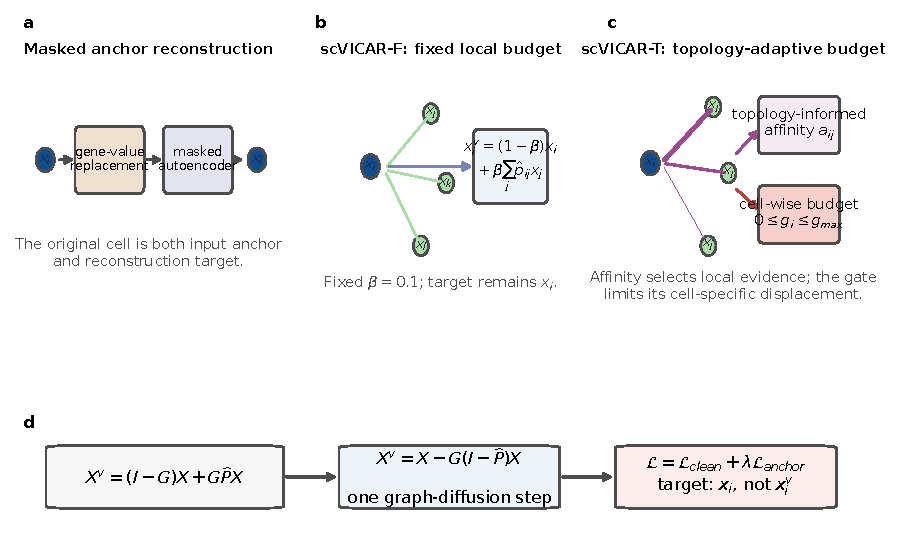
\includegraphics[width=\textwidth]{fig1_method.pdf}
  \caption{scVICAR 方法框架。scVICAR-F 使用固定混合系数构造有界邻域视图；scVICAR-T 增加拓扑信息亲和度和逐细胞混合系数。两种变体均从邻域破坏视图恢复原始锚点。}
  \label{fig:zh-1}
\end{figure*}

设预处理表达矩阵为 $X=[x_1,\ldots,x_n]^\top\in\mathbb{R}^{n\times d}$。scVICAR 将静态细胞图转换为有界训练视图，然后通过掩码骨干恢复未经修改的锚点。真实标签不参与干净预处理、图构建、表征学习和模型选择。唯一例外是独立的压力实验，其中标签仅用于构造预先规定的跨类别替换边。

\subsection{3.1 预处理与共同骨干}

对于计数型输入，每个细胞归一化到 $10^4$ 的文库大小，随后执行 $\log(1+x)$。选择 1,000 个 Seurat 风格高变基因并逐基因标准化。如果有限的归一化离散度不足 1,000 个，则使用确定性的经验方差回退方案，确保恰好保留 1,000 个基因。

所有骨干匹配实验共享相同的三层编码器、掩码预测器、线性解码器、优化器、训练预算和预处理。编码器宽度为 $256\rightarrow128\rightarrow128$，线性头预测 $d$ 维破坏掩码，解码器从潜变量与掩码 logits 的拼接向量中重建表达。

对 minibatch $X_B$，设 $M$ 为 Bernoulli 掩码，$\Pi$ 为 batch 的随机排列，则 scMAE 破坏为

\begin{equation}
C_{M,\Pi}(X_B)=(1-M)\odot X_B+M\odot\Pi X_B.
\end{equation}

由于替换值可能恰好等于原值，监督掩码采用实际变化指示量 $\widetilde M=\mathbf 1[C_{M,\Pi}(X_B)\neq X_B]$。该指示量记录 Bernoulli 抽样后实际发生的变化。骨干损失由加权重建误差和掩码二元交叉熵组成。冻结协议设置 $\lambda_x=0.75$、$\lambda_m=0.7$。

\subsection{3.2 静态细胞图}

在 50 维 PCA 表征上进行行归一化，并构建 $k=5$ 的有向余弦 KNN 图。对 $j\in\mathcal N_i$，定义余弦相似度 $s_{ij}$ 和距离 $d_{ij}=1-s_{ij}$。基础转移概率为

\begin{equation}
p_{ij}^{(0)}=\frac{\exp(s_{ij}/\tau)}{\sum_{\ell\in\mathcal N_i}\exp(s_{i\ell}/\tau)},\qquad \tau=0.2.
\end{equation}

图在训练前只构建一次，不随学习到的 embedding 动态更新。实现中有放回地抽取 $m=4$ 个邻居位置，并按抽样亲和度再次加权。该采样后重加权估计器被忠实保留，但不被宣称为全邻域加权平均的无偏估计。无偏随机平均与全邻域聚合仅作为机制消融。

\subsection{3.3 scVICAR-F：固定邻域破坏}

对锚点 $i$，邻域聚合为 $\bar x_i=\sum_j\widehat p_{ij}x_j$。scVICAR-F 构造

\begin{equation}
x_i^v=(1-g)x_i+g\bar x_i,\qquad g=0.1.
\end{equation}

这对应原 NeighborMix 中的 $\alpha=0.9$。$x_i^v$ 作为输入视图，原始细胞 $x_i$ 始终是恢复目标。该分支随后接受与主干相同的基因替换破坏。我们将这一训练方式称为图邻域锚点恢复。

\subsection{3.4 scVICAR-T：拓扑自适应破坏}

scVICAR-T 解决不同细胞的局部图一致性不同、统一扰动幅度可能不合适的问题。令 $m_{ij}$ 表示互惠 KNN，令共享最近邻重叠为

\begin{equation}
q_{ij}^{\mathrm{SNN}}=\frac{|\mathcal N_i\cap\mathcal N_j|}{|\mathcal N_i\cup\mathcal N_j|}.
\end{equation}

未归一化拓扑信息亲和度为

\begin{equation}
a_{ij}\propto p_{ij}^{(0)}e^{\gamma_s s_{ij}}(1+\gamma_m m_{ij})
(1+\gamma_q q_{ij}^{\mathrm{SNN}})e^{-\gamma_d d_{ij}}.
\end{equation}

冻结协议设置 $\gamma_s=\gamma_m=\gamma_q=\gamma_d=1$。

逐细胞混合系数综合互惠邻居比例、平均 SNN 重叠和相似度加权扰动代理：

\begin{equation}
g_i=g_{\min}+(g_{\max}-g_{\min})
\sigma(\beta_m\bar m_i+\beta_q\bar q_i-\beta_\rho\rho_i).
\end{equation}

冻结协议设置 $g_{\min}=0$、$g_{\max}=0.1$、$\beta_m=\beta_q=1$、$\beta_\rho=2$。该表达式不包含不确定性估计、学习型 gate、聚类分配、标签或动态图。

\subsection{3.5 统一目标与推理}

令 $G=\operatorname{diag}(g_1,\ldots,g_n)$，两种变体统一写为

\begin{equation}
X^v=(I-G)X+G\widehat PX=X-G(I-\widehat P)X.
\end{equation}

scVICAR-F 使用 $G=0.1I$，scVICAR-T 使用逐细胞混合系数。总损失由干净 scMAE 损失和加权邻域恢复损失组成，邻域损失权重固定为 $\lambda_v=0.3$。推理时将干净矩阵直接输入编码器，聚类在获得 embedding 后执行。

所有匹配变体均训练 80 个 epoch，batch size 为 256，学习率为 $10^{-3}$，掩码比例为 0.4，embedding 维度为 128。NoMix 设置 $G=0$ 且 $\lambda_v=0$；edge-only、gate-only 和 RandomMix 分别用于隔离不同设计因素。

\section{4. 理论分析}

\subsection{4.1 凸包与位移上界}

当 $\widehat P$ 非负且行随机，并且 $0\le g_i\le1$ 时，每个邻域视图满足

\begin{equation}
x_i^v\in\operatorname{conv}\bigl(\{x_i\}\cup\{x_j:\widehat p_{ij}>0\}\bigr).
\end{equation}

若 $R_i=\max_{j:\widehat p_{ij}>0}\|x_j-x_i\|_2$，则

\begin{equation}
\|x_i^v-x_i\|_2\le g_i\sum_j\widehat p_{ij}\|x_j-x_i\|_2
\le g_{\max}R_i.
\end{equation}

因此，视图不会离开锚点及其采样邻居构成的局部凸包，其最大位移受到 gate 和邻域半径共同限制。若编码器 $h$ 在局部凸包上为 $L_h$-Lipschitz，则

\begin{equation}
\|h(x_i^v)-h(x_i)\|_2\le L_hg_iR_i.
\end{equation}

该式只是扰动传播上界，不证明训练一定得到不变或更可分的表征。

\subsection{4.2 一步非均匀图扩散}

令随机游走拉普拉斯 $L_{\mathrm{rw}}=I-\widehat P$，则

\begin{equation}
X^v=X-GL_{\mathrm{rw}}X.
\end{equation}

该视图相当于采用节点相关步长的一次显式 Euler 扩散。当 $G=gI$ 且核对称或可逆时，特征值为 $\lambda_r$ 的图频率成分被乘以 $1-g\lambda_r$。这提供了有条件的低通解释，同时提示过平滑风险。scVICAR 在每个训练视图上应用一次该操作。

\subsection{4.3 对数线性拓扑核}

在 $d_{ij}=1-s_{ij}$ 且裁剪未激活时，亲和度可以写为 softmax 形式：

\begin{equation}
r_{ij}=(\tau^{-1}+\gamma_s+\gamma_d)s_{ij}
+\log(1+\gamma_m m_{ij})+\log(1+\gamma_q q_{ij}^{\mathrm{SNN}}),
\end{equation}

\begin{equation}
a_{ij}=\frac{\exp(r_{ij})}{\sum_{\ell\in\mathcal N_i}\exp(r_{i\ell})}.
\end{equation}

该亲和度是乘积专家或对数线性的图评分。余弦相似度和余弦距离在这里存在代数冗余，所得边权未经概率校准。

\subsection{4.4 跨类别邻域污染}

仅用于事后分析时，将邻居划分为同类集合 $S_i$ 和跨类集合 $C_i$，并定义错误邻居权重质量 $\eta_i=\sum_{j\in C_i}\widehat p_{ij}$。若同类和跨类半径分别由 $R_i^{\mathrm{in}}$ 和 $R_i^{\mathrm{out}}$ 限制，则

\begin{equation}
\|x_i^v-x_i\|_2\le g_i\bigl[(1-\eta_i)R_i^{\mathrm{in}}+\eta_iR_i^{\mathrm{out}}\bigr].
\end{equation}

当 $R_i^{\mathrm{out}}\ge R_i^{\mathrm{in}}$ 时，减少 $\eta_i$ 会单调收紧上界；减小 $g_i$ 会收缩整个扰动，但不会改变错误边质量。因此，拓扑自适应只有在亲和度或 gate 对错误结构作出有利响应时才可能产生优势，这一优势并非对任意 KNN 图都成立。

\subsection{4.5 条件性局部风险解释}

对固定模型参数、minibatch 上下文和锚点，考虑破坏平均后的条件风险。对邻域位移进行 Taylor 展开后，风险包括一阶方向项、由 $\mathbb E[\delta_i\delta_i^\top]$ 决定的二阶曲率项，以及三阶余项。只有当采样扰动近似中心化，或输入方向梯度较小时，一阶项才可忽略。在此额外条件下，二阶项具有图支撑的方向曲率正则化解释。进一步假设平方重建残差较小时，它才近似于方向性 Jacobian 惩罚。本文不以该展开证明聚类性能必然提高。

上述理论给出三个经验预测：随机混合不应复现局部几何的全部行为；降低跨类别权重质量应改善污染上界；当不同锚点的局部纯度差异较大时，逐细胞收缩应更有价值。RandomMix、错误邻边曲线、affinity AUROC 和 gate–purity 关联分别检验这些预测。

\section{5. 实验协议}

\subsection{5.1 证据设计与数据集}

评价分别回答广度、归因、机制和效用问题。开发阶段基准覆盖 15 个有效数据集、17 个完整方法配置和 3 个随机种子。每个配置完成 45 次运行，主比较共包含 765 次成功且非回退的运行。scVICAR-F 和 scVICAR-T 的最终参数在该阶段确定，因此该基准用于评价广泛竞争力。确认性队列包含六个随后冻结的数据集：Blood–Bone Marrow、Human Pancreas 1、Human Pancreas 3、Mouse Pancreas 1、PRJNA895163 和 Tabula Sapiens Pancreas。

更广的轻量级实验归档记录了 22 个外部或骨干模型的 1,055 条运行记录，其中 749 条成功、168 条失败、97 条回退、41 条待完成。主排名仅纳入在 15 个有效数据集上覆盖完整的配置；覆盖不完整或产生回退输出的 8 个实现连同状态统计在补充材料中披露。

主分析删除标准化标签为 \texttt{unknown}、\texttt{nan} 或 \texttt{unassigned} 的细胞，并删除少于 10 个细胞的类别。完整标签结果作为独立敏感性分析。\texttt{hrvatin\_geo} 因标签语义无效而排除，也不与 \texttt{hrvatin} 作为两个独立数据集计数。每个确认性 H5AD 均由 SHA-256 唯一标识。

\subsection{5.2 匹配变体和基线}

共同骨干下比较 NoMix、RandomMix、scVICAR-F、topology edge-only、topology gate-only 和完整 scVICAR-T。外部基线包括 PCA+KMeans、Original scMAE、scVI、scDeepCluster、scDCC 和 scRCL。只有当数据哈希和全部评价字段完全一致时才复用历史结果，否则重新运行。scDCC、scDeepCluster 和 scRCL 的原始架构在训练时需要已知 $K$，因此明确标记为 known-$K$ training baselines；逐细胞真实标签仍不进入梯度更新和 checkpoint 选择。

\subsection{5.3 评价与冻结超参数}

模型种子为 42、2024 和 3407。六个数据集、六个匹配变体和三个种子构成 108 次主要运行。主要终点是已知 $K$、\texttt{n\_init=20} 的 KMeans ARI。NMI、assignment accuracy、macro-F1、silhouette、运行时间和峰值显存为次要指标。固定分辨率 1.0 的 Leiden 单独报告，不允许标签引导的分辨率搜索。

图参数为 $k=5$、抽样邻居数 4、$\tau=0.2$、最大 gate 0.1。模型训练 80 个 epoch，batch size 256，学习率 $10^{-3}$，mask ratio 0.4，邻域损失权重 0.3。不做逐数据集调参，也不启用 uncertainty、动态图、学习型 gate 或显式 consistency loss。

\subsection{5.4 图污染与统计分析}

在 Blood–Bone Marrow、Human Pancreas 3 和 PRJNA895163 上，将每个图行的 0\%、25\%、50\%、75\% 或 100\% 邻边替换为跨类别邻居。标签只用于构造该压力干预，不进入干净实验。除比较 F/T 的绝对性能外，还比较相对 0\% 污染的退化量。聚合器消融包括当前采样后重加权、无偏随机平均和全邻域聚合。

数据集是独立统计单位。下游 split seeds 先在模型运行内部平均，模型 seeds 再在数据集内部平均。预设对比为 F–NoMix、T–NoMix 和 T–F。报告数据集配对效应、胜/平/负、层级 bootstrap 95\% 置信区间、配对符号翻转置换检验及 Holm 校正。细胞、拆分和随机种子不被视为独立生物学重复，也不选择最佳种子。

\section{6. 聚类与鲁棒性结果}

\subsection{6.1 十五数据集大规模基准}

排除标签语义无效的 \texttt{hrvatin\_geo} 后，正式开发基准包含 15 个数据集、17 个完整方法配置和每个数据集 3 个随机种子，共 765 次成功且非回退的运行。scVICAR-T 在 ACC、NMI、ARI 和 macro-F1 四项平均指标上均排名第一，scVICAR-F 在四项指标上均排名第二。scVICAR-T、scVICAR-F 和 scMAE 的平均 ARI 分别为 0.7955、0.7868 和 0.7570；两种 scVICAR 相对 scMAE 的提升分别为 5.08\% 和 3.93\%。表现最好的其他方法 scNAME 的平均 ARI 为 0.7326，scVICAR-T 和 scVICAR-F 分别高 8.59\% 和 7.40\%。

按数据集汇总后，scVICAR-T 在 15 个数据集中的 10 个超过 scMAE，ARI 变化中位数为 +0.0152；它在 11 个数据集上进入前三，并在 4 个数据集上排名第一。scVICAR-F 在 9 个数据集上超过 scMAE，ARI 变化中位数为 +0.0019。scVICAR-T 在 Shekhar、Macosko、Quake Smart-seq2 Lung 和 Baron 上获得较大增益；worm neuron、Young 和 Bach 更有利于 scMAE。该基准同时展示总体排名与数据集差异。最终 F/T 配置在这一阶段确定，因此后续六数据集评估承担外部有效性验证。

\subsection{6.2 冻结外部竞争力}

在六个冻结数据集的外部比较中，scVICAR-T 的平均 ARI 为 0.617，是所比较方法中的最高值。它比 Original scMAE 高 2.13\%，比 PCA+KMeans 高 5.11\%，比 scDCC 高 11.17\%，比 scDeepCluster 高 21.46\%，比 scRCL 高 17.75\%，比 scVI 高 44.16\%。scVICAR-F 获得最高平均 NMI 和 macro-F1。该比较评价采用不同骨干、目标和实现的完整方法。随后使用 matched-backbone 分析估计邻域混合本身的作用。

\subsection{6.3 骨干匹配归因}


\begin{figure*}[t]
  \centering
  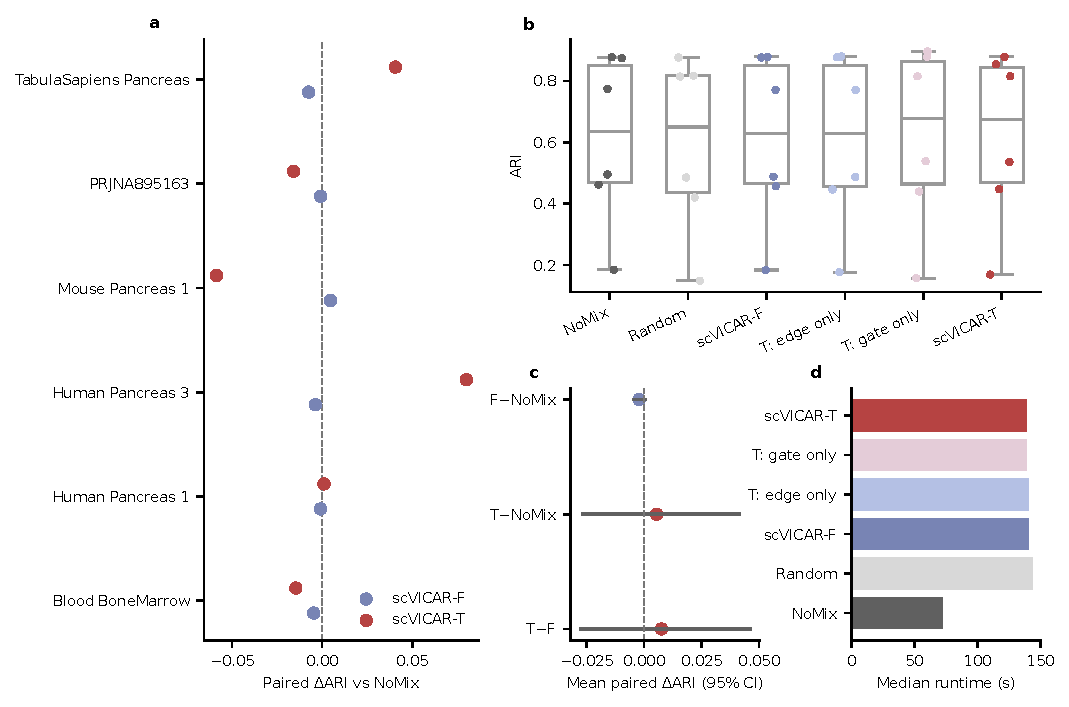
\includegraphics[width=\textwidth]{fig2_confirmatory.pdf}
  \caption{六个冻结数据集上的骨干匹配比较。图中给出相对 NoMix 的数据集层面 ARI 变化、变体分布、预设配对效应及共同训练预算下的运行时间。}
  \label{fig:zh-2}
\end{figure*}

108 次冻结主要运行全部完成。在预处理、架构、优化器、训练预算和种子计划均相同的条件下，scVICAR-F 相对 NoMix 的平均 ARI 变化为 −0.002，胜/平/负为 1/0/5；scVICAR-T 的变化为 +0.005，胜/平/负为 3/0/3。两个数据集层面的置信区间均跨越零。Human Pancreas 3 的自适应增益最大，另一些数据集则更有利于 NoMix。

外部排名反映完整训练流程。在共同骨干内部，corruption design 带来幅度较小且依赖数据集的正则化效应。

\subsection{6.4 组件证据与负对照}


\begin{figure*}[t]
  \centering
  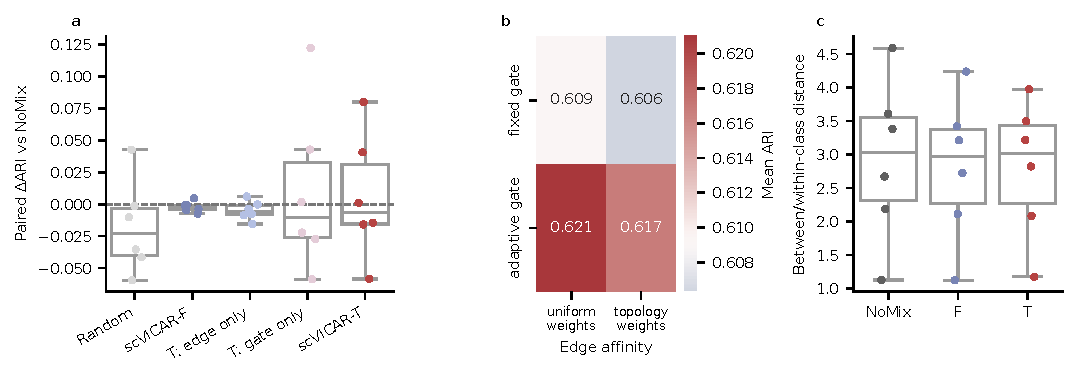
\includegraphics[width=\textwidth]{fig3_components.pdf}
  \caption{组件与负对照实验。RandomMix、固定邻域破坏、拓扑边权、逐细胞混合系数及完整模型使用相同骨干与训练预算。}
  \label{fig:zh-3}
\end{figure*}

RandomMix 的描述性平均 ARI 最低，为 0.594，低于 NoMix 的 0.611，说明邻居选择会影响结果。Topology edge-only 的平均 ARI 为 0.606。Gate-only 得到最高描述性平均 ARI 0.621，完整 scVICAR-T 为 0.617。在这些干净图上，逐细胞混合系数是表现更好的自适应组件。Gate-only 位于预设推断对比之外，因此这里报告描述性排序。

当前实现中，邻域变体的运行时间约为 NoMix 的两倍。

\subsection{6.5 标签保留与聚类器敏感性}

完整标签敏感性分析保留所有来源标签和细胞，共 54 次独立冻结运行。scVICAR-T 相对 NoMix 的平均 ARI 提高 0.030，并在 5/6 数据集上占优；95\% 区间仍跨越零。该结果提示，当稀有或未解析群体被保留时，拓扑自适应可能更加重要。专门的 rare-cell 实验可以进一步检验这一解释。

固定分辨率 Leiden 改变了绝对得分和部分排序。scVICAR-F 相对 NoMix 的平均 ARI 变化为 +0.012，scVICAR-T 为 +0.002，区间均跨越零。这一结果说明方法排序对聚类算子存在一定依赖。

\subsection{6.6 拓扑评分能够检测错误邻边风险}


\begin{figure*}[t]
  \centering
  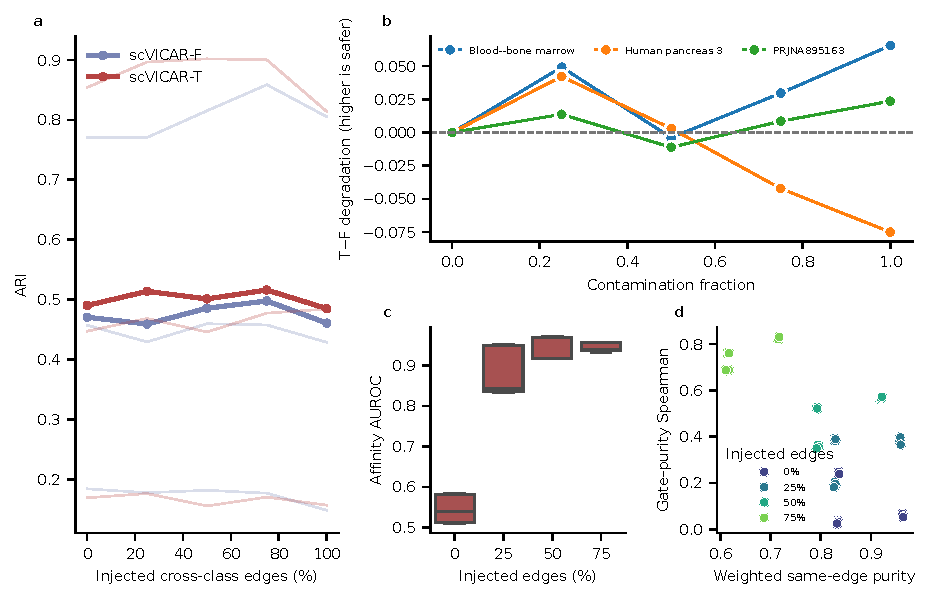
\includegraphics[width=\textwidth]{fig4_graph_stress.pdf}
  \caption{三个数据集上的受控图污染实验。结果包括 ARI 退化曲线、scVICAR-T 与 scVICAR-F 的相对响应、边亲和度 AUROC 及逐细胞混合系数与邻域纯度的关联。}
  \label{fig:zh-4}
\end{figure*}

压力实验直接检验理论污染上界所指出的量。拓扑信息亲和度区分同类保留边和注入跨类别边的平均 AUROC 为 0.918。逐细胞混合系数与加权邻域纯度的平均 Spearman 相关系数为 0.520，说明两个自适应组件会响应其对应的图属性。

在 100\% 错误邻边条件下，scVICAR-T 在 2/3 数据集上退化更慢，scVICAR-F 在 1/3 数据集上更好。拓扑评分能够识别污染，其对 ARI 的影响取决于数据集和受污染图的几何结构。

\section{7. 下游预测效用与标记基因一致性}

聚类一致性无法说明 embedding 是否保留了注释信号或簇层面的基因程序。因此，我们区分两类结果：冻结线性探针衡量低标签量线性可分性，marker 任务衡量不使用评价标签构造簇 marker 时的生物学一致性。

\subsection{7.1 Marker recovery}

每个数据集按照 50\% reference / 50\% evaluation 分层拆分，并使用五个固定拆分种子。reference cells 根据真实类型通过 Wilcoxon 得到每类 top-100 markers。evaluation cells 仅根据预测簇独立计算 marker，真实 evaluation 标签不参与差异表达。报告 Recovery@20/@50/@100、Jaccard、overlap coefficient 及无有效 marker 簇的比例。

\subsection{7.2 Marker-overlap annotation}

每个预测簇被分配给 reference marker overlap 最大的类型，允许多个簇对应同一类型。并列时先比较共享 marker 的平均 log fold change，再按类型名排序。marker 少于 3 个或最大 overlap 为 0 的簇记为 \texttt{unassigned}。Hungarian mapping 仅作为 oracle upper bound，不作为实际注释方法。

\subsection{7.3 低标签量冻结 embedding 探针}

在 10\% 和 30\% 标签比例下，使用分层抽样训练 \texttt{StandardScaler + L2 multinomial logistic regression}。参数为 $C=1$、balanced class weights、最大迭代 2,000 次。Scaler 和分类器仅在训练子集上拟合，encoder 始终冻结。该任务衡量数据集内部的 transductive annotation。

\subsection{7.4 结果}


\begin{figure*}[t]
  \centering
  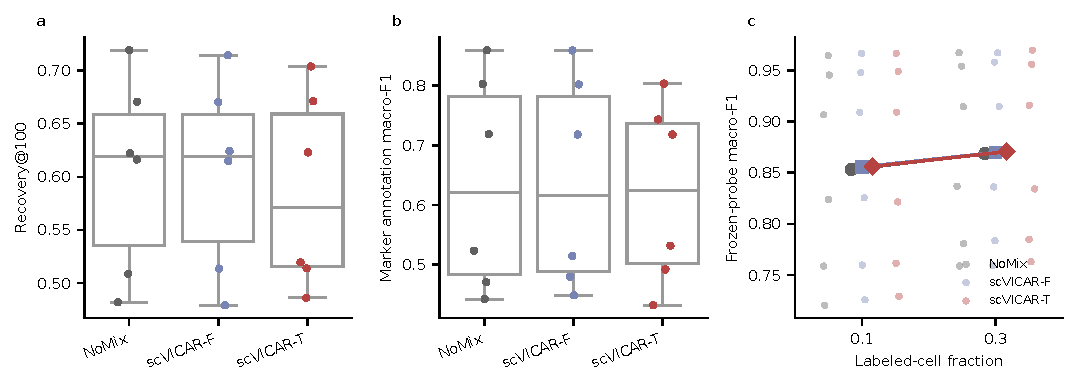
\includegraphics[width=\textwidth]{fig5_downstream.pdf}
  \caption{六个冻结数据集上的下游效用。图中分别报告 marker recovery、marker-overlap annotation 和低标签量冻结表征线性探针。}
  \label{fig:zh-5}
\end{figure*}

最一致的下游信号来自低标签量探针。在 10\% 标签下，scVICAR-F 在全部六个数据集上超过 NoMix，scVICAR-T 在五个数据集上超过 NoMix；相对 macro-F1 增益分别为 0.29\% 和 0.34\%。在 30\% 标签下，相对增益分别为 0.13\% 和 0.22\%。这些变化方向较一致，绝对幅度很小；所有 Holm 校正后的预设检验均高于 0.05。

Marker 终点给出了不同结果。scVICAR-T 相对 NoMix 的 Recovery@100 平均变化为 −0.0168，marker annotation macro-F1 平均变化为 −0.0162，两个区间均跨越零。线性可分性的小幅变化与异质的簇层面 marker 结果同时出现。

\subsection{7.5 Human Pancreas 3 案例}


\begin{figure*}[t]
  \centering
  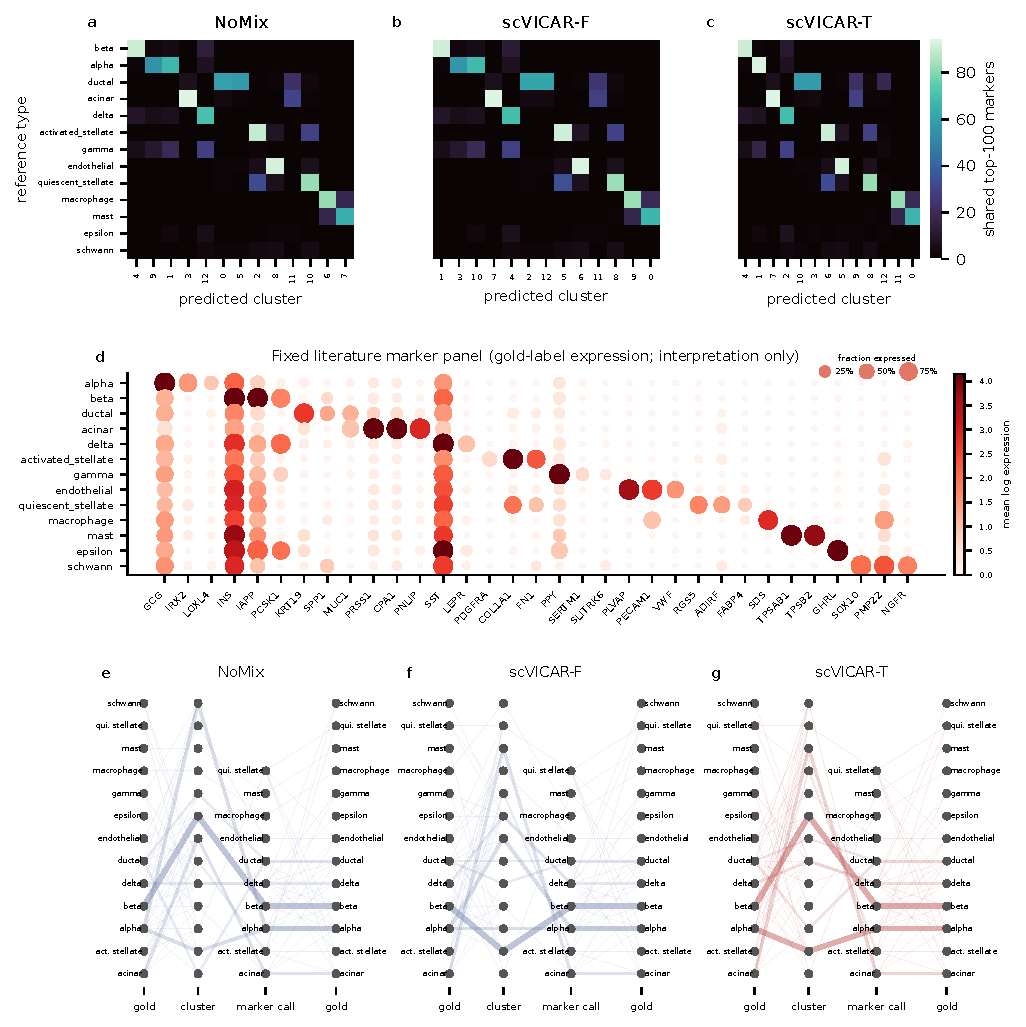
\includegraphics[width=\textwidth]{fig6_pancreas_case.pdf}
  \caption{Human Pancreas 3 预设案例。图中比较 NoMix、scVICAR-F 和 scVICAR-T 的 marker overlap、文献核验 marker panel 及类型到聚类和注释的对应关系。}
  \label{fig:zh-6}
\end{figure*}

该案例在查看 marker 前固定比较 NoMix、scVICAR-F 和 scVICAR-T，并使用固定的模型种子 42 与 downstream split seed 11。图中包括类型—簇 marker overlap、经文献核验的胰腺 marker panel，以及 reference type → cluster → marker annotation → gold type 的 Sankey 流程。文献 marker 只用于解释，不进入训练、图构建或模型选择。

\section{8. 讨论与局限}

scVICAR 使用细胞间结构构造训练输入。解码器恢复原始细胞，推理时编码器直接处理干净表达谱。该设计只在训练阶段增加一次图操作，凸包和位移上界描述了输入发生的变化。

完整 scVICAR 流程在所评估数据上表现较好。在 15 个开发数据集的 17 个完整配置中，scVICAR-T 和 scVICAR-F 在四项平均指标上分别位列第一和第二。按数据集计算，scVICAR-T 在 10/15 个数据集上超过 scMAE，并在 11/15 个数据集上进入前三。在六个冻结数据集上，scVICAR-T 获得最高平均 ARI，scVICAR-F 获得最高平均 NMI 和 macro-F1。骨干匹配条件下，scVICAR-F 和 scVICAR-T 相对 NoMix 的平均 ARI 变化分别为 −0.002 和 +0.005。外部排名描述完整训练流程，骨干匹配效应估计局部混合的增量贡献；该贡献随数据集变化。

消融说明了各组件的作用。RandomMix 低于局部混合，表明邻居选择会影响结果。gate-only 的描述性干净图 ARI 最高，edge-only 则低于 NoMix。在这些干净确认图上，逐细胞控制混合强度是更有效的自适应组件。

压力实验直接测量了拓扑组件的响应。拓扑信息亲和度识别跨类别边的平均 AUROC 为 0.918，逐细胞混合系数与加权邻域纯度的平均 Spearman 相关系数为 0.520。在完全替换邻边时，ARI 退化在两个数据集上有利于 scVICAR-T，在一个数据集上有利于 scVICAR-F。图几何和编码器对混合输入的响应共同决定最终聚类变化。

下游任务呈现出较具体的模式。冻结低标签量探针的相对 macro-F1 提升为 0.13\%–0.34\%，多数数据集为正向变化。Marker recovery 和 marker-overlap annotation 的变化更大，scVICAR-T 在两个 marker 指标上的平均变化为负。局部混合对线性类别分离的影响更一致，但没有一致改善簇层面的 marker coherence。较高的基线 probe 准确率和数据集特异的 marker 质量也会限制可观察增益。

当前方法使用静态 PCA 余弦 KNN 图，因此过渡状态、批次边界和稀有群体附近可能出现跨类型邻边。拓扑信息亲和度是未经校准的解析权重。当前公式中的余弦相似度与余弦距离存在代数冗余。采样器还使用同一亲和度完成抽样和重加权，使有效核更加尖锐。替代估计器在零注入污染下得到相近的平均 ARI。

本研究覆盖六个冻结数据集、三个模型种子、已知 $K$ 的 KMeans 和固定分辨率 Leiden。其他组织、疾病状态、平台和批次结构可能产生不同的图错误。完整标签敏感性结果提示稀有或未解析群体可能受益，后续可使用专门的 rare-cell 设计检验。低标签量探针衡量的是数据集内部的传导式注释。在这一范围内，scVICAR 提供了具有竞争力的掩码表征，并量化了局部图质量对邻域混合的影响。

\section{9. 数据与代码可用性}

本文使用的数据均来自正文所引用的公共来源和 accession。考虑不同数据源的再分发条款，确认性分析使用的处理后 H5AD 不随论文直接再分发。复现包记录来源标识、预处理和过滤规则、数据维度及 SHA-256，以便重建和核验输入。

双盲评审包包含模型、评价、聚合、统计分析和作图代码，以及冻结配置清单。每个结果都关联唯一 run identifier、配置哈希、代码冻结标识和文件级校验和。最终论文发布时将同步提供归档版本；在正式归档前不虚构仓库链接。

\section{10. 结论}

本文提出 scVICAR：模型从有界的邻域混合输入中恢复原始细胞。scVICAR-F 使用固定混合系数，scVICAR-T 根据局部图结构调整边权和逐细胞混合系数。凸包、扩散和污染分析描述了这些操作对输入的影响。

scVICAR-T 和 scVICAR-F 在 15 数据集开发基准的四项平均指标上分别位列第一和第二；scVICAR-T 也在六数据集冻结外部比较中获得最高平均 ARI。骨干匹配对照显示，局部混合的增量作用较小且依赖数据集。受控错误邻边替换表明自适应评分能够识别不可靠邻边，最终 ARI 变化随数据集而异。低标签量探针呈小幅正向变化，marker 指标则具有异质性。这些结果给出了邻域混合锚点恢复在单细胞表征学习中的适用范围。

---

\end{document}
